\cotefile{64}
\scanpage{78}
\mspage{3}

où $Q_0$ est un carré donné une fois pour toutes ($\unsure{h|k}$ étant fixé\deleted{\unsure{)|?}}, disons, quand même), ou comme seule donnée un iso

\[
\underline{\omega}_{Q_0}\deleted{\unsure{(Q_0)|Q_0}}\simeq\mu_4^*
\qquad\text{i.e. d'un élément du }\mu_4^*\wedge\underline{\omega}_{Q_0}
\tag*{(16)}
\]

i.e. un isom.

\[
\mu_4^{\deleted{\unsure{*}}}\simeq\mathrm{Aut}^+(Q_0)\,.
\tag*{(17)}
\]

Pour des raisons qui apparaîtront par la suite, le choix le plus opportun est de prendre pour $Q_0$ le carré \deleted{\unsure{dont|tout} satisfaisant} \inserted{à \unsure{donner|donnée|donné}} (17), avec un coté fixé, dont \deleted{les extrémités} \inserted{\unsure{l'ens|l'un|l'ens.} des sommets incidents} $s,s'$ \deleted{sont} donc en corr. biunivoque avec l'ens $\mu_4^*=\{i,i'\}$ des racines carrées de $-1$, par la condition que

\figure{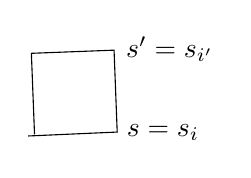
\begin{tikzpicture}[x=1cm,y=1cm]
\draw (0.04,0) -- (0,1.03) -- (1.05,1.07) -- (1.09,0.03) -- (-0.04,-0.02);
\node[anchor=west] at (1.08,1.08) {$s'=s_{i'}$};
\node[anchor=west] at (1.09,0.02) {$s=s_i$};
\end{tikzpicture}}

\[
\deleted{\unsure{s'|i'}\quad s'=i_s s}
\]

\[
\deleted{\unsure{s=is|s'=is}}\;s_{i'}=i\,s_i\qquad\text{d'où}\quad s_i=i's_{i'}
\tag*{(18)}
\]

puisque $i'=i^{-1}=-i$. Ainsi, $T_0$ peut s'interpréter comme muni de la structure \deleted{\unsure{que|qui}} \inserted{suivante, qui le caractérise~:} $T_0\otimes\underline{O}_{t}(-1)$ est muni d'une paire de bases, \deleted{reliées entre} \inserted{en corr. $1$-$1$} avec $\mu_4^*$, satisfaisant les $=$.s relations (18):, où maintenant le produit $i\,s_i$ est au sens de la structure vectorielle de $T_0\otimes\underline O_t(-1)$. \deleted{\unsure{Si}}

Ici on aura un iso. canonique

\[
D_{Q_0}\simeq\mu_4^*
\tag*{(19)}
\]

et par suite la donnée (16) équivaut à la donnée d'un iso
% archive sheet number: 77
